\documentclass{article}
\usepackage{physics}
\usepackage{graphicx}
\usepackage{caption}
\usepackage{amsmath}
\usepackage{bm}
\usepackage{framed}
\usepackage{authblk}
\usepackage{empheq}
\usepackage{amsfonts}
\usepackage{esint}
\usepackage[makeroom]{cancel}
\usepackage{dsfont}
\usepackage{centernot}
\usepackage{mathtools}
\usepackage{bigints}
\usepackage{amsthm}
\theoremstyle{definition}
\newtheorem{defn}{Definition}[section]
\newtheorem{prop}{Proposition}[section]
\newtheorem{rmk}{Remark}[section]
\newtheorem{thm}{Theorem}[section]
\newtheorem{exmp}{Example}[section]
\newtheorem{prob}{Problem}[section]
\newtheorem{sln}{Solution}[section]
\newtheorem*{prob*}{Problem}
\newtheorem{exer}{Exercise}[section]
\newtheorem*{exer*}{Exercise}
\newtheorem*{sln*}{Solution}
\usepackage{empheq}
\usepackage{tensor}
\usepackage{xcolor}
%\definecolor{colby}{rgb}{0.0, 0.0, 0.5}
\definecolor{MIT}{RGB}{163, 31, 52}
\usepackage[pdftex]{hyperref}
%\hypersetup{colorlinks,urlcolor=colby}
\hypersetup{colorlinks,linkcolor={MIT},citecolor={MIT},urlcolor={MIT}}  
\usepackage[left=1in,right=1in,top=1in,bottom=1in]{geometry}

\usepackage{newpxtext,newpxmath}
\newcommand*\widefbox[1]{\fbox{\hspace{2em}#1\hspace{2em}}}

\newcommand{\p}{\partial}
\newcommand{\R}{\mathbb{R}}
\newcommand{\C}{\mathbb{C}}
\newcommand{\lag}{\mathcal{L}}
\newcommand{\nn}{\nonumber}
\newcommand{\ham}{\mathcal{H}}
\newcommand{\M}{\mathcal{M}}
\newcommand{\I}{\mathcal{I}}
\newcommand{\K}{\mathcal{K}}
\newcommand{\F}{\mathcal{F}}
\newcommand{\w}{\omega}
\newcommand{\lam}{\lambda}
\newcommand{\al}{\alpha}
\newcommand{\be}{\beta}
\newcommand{\x}{\xi}
\def\dbar{{\mkern3mu\mathchar'26\mkern-12mu   d}}


\newcommand{\G}{\mathcal{G}}

\newcommand{\f}[2]{\frac{#1}{#2}}

\newcommand{\ift}{\infty}

\newcommand{\lp}{\left(}
\newcommand{\rp}{\right)}

\newcommand{\lb}{\left[}
\newcommand{\rb}{\right]}

\newcommand{\lc}{\left\{}
\newcommand{\rc}{\right\}}


\newcommand{\V}{\mathbf{V}}
\newcommand{\U}{\mathcal{U}}
\newcommand{\Id}{\mathcal{I}}
\newcommand{\D}{\mathcal{D}}
\newcommand{\Z}{\mathcal{Z}}

%\setcounter{chapter}{-1}



\usepackage{enumitem}


\usepackage{subfig}
\usepackage{listings}
\captionsetup[lstlisting]{margin=0cm,format=hang,font=small,format=plain,labelfont={bf,up},textfont={it}}
\renewcommand*{\lstlistingname}{Code \textcolor{violet}{\textsl{Mathematica}}}
\definecolor{gris245}{RGB}{245,245,245}
\definecolor{olive}{RGB}{50,140,50}
\definecolor{brun}{RGB}{175,100,80}

%\hypersetup{colorlinks,urlcolor=colby}
\lstset{
	tabsize=4,
	frame=single,
	language=mathematica,
	basicstyle=\scriptsize\ttfamily,
	keywordstyle=\color{black},
	backgroundcolor=\color{gris245},
	commentstyle=\color{gray},
	showstringspaces=false,
	emph={
		r1,
		r2,
		epsilon,epsilon_,
		Newton,Newton_
	},emphstyle={\color{olive}},
	emph={[2]
		L,
		CouleurCourbe,
		PotentielEffectif,
		IdCourbe,
		Courbe
	},emphstyle={[2]\color{blue}},
	emph={[3]r,r_,n,n_},emphstyle={[3]\color{magenta}}
}






\begin{document}
		\begin{framed}
			\noindent Name: \textbf{Huan Q. Bui}\\
			Course: \textbf{8.333 - Statistical Mechanics I}\\
			Problem set: \textbf{\#5}
		\end{framed}
	



\noindent \textbf{1. Repulsive shell potential.} The potential is 
\begin{align*}
\mathcal{V}(r) = \begin{cases}
0, \quad 0 < r < a,\\
u, \quad a < r < b,\\
0, \quad b < r < \infty
\end{cases}
\end{align*}

\begin{enumerate}[label=(\alph*)]
	\item 
	\begin{align*}
	B_2(T) = -\f{b_2}{2} = -\f{1}{2}\int_{\mathbb{R}^3} d^3 \vec{r} \lp e^{-\be \mathcal{V}(r)} - 1 \rp = -2\pi \int_a^b \,dr r^2 \lp e^{-\be u} - 1 \rp = \boxed{-\f{2\pi}{3} \lp e^{-\be u } - 1 \rp (b^3 - a^3)}
	\end{align*}
	\item The equation of state is 
	\begin{align*}
	\f{P}{k_B T} = \f{N}{V}\lp 1 + B_2(T) \f{N}{V} \rp \implies PV \lp 1 + B_2(T)\f{N}{V} \rp^{-1} = N k_B T
	\end{align*}
	In the low density limit where $N/V \equiv n \ll 1$, we have
	\begin{align*}
	\lp 1 + B_2(T) \f{N}{V}  \rp^{-1} = \lp 1 + B_2(T) \f{N}{V}\rp^{-1} \approx 1 - B_2(T) \f{N}{V}
	\end{align*}
	with which we set the LHS to be equal to $P(V-N\Omega)$ and find that 
	\begin{align*}
	\boxed{\Omega = -\f{2\pi}{3} (b^3 - a^3) \lp e^{-\be u} - 1  \rp }
	\end{align*}
	
	
	\item 
	\begin{align*}
	\Omega_\text{hard shell} = \lim_{u\to \infty} \Omega = \boxed{\f{2\pi}{3} (b^3 - a^3) }
	\end{align*}
	I suppose the dependence on $a$ makes sense. When $a=0$, we get the result for hard-sphere potential. When $a\neq 0$ like this case, the excluded volume is smaller since the potential acts on a more limited range. \textbf{\textcolor{blue}{Not sure how to interpret what happens inside the shell... I guess once a particles makes it inside the shell, it gets trapped there since there is no repulsion.}} However, if we think about the low density limit, then particles are far apart, and the excluded volume shouldn't depend on $a$, so in this case the dependence does not make sense.
\end{enumerate}

\noindent \textbf{2. Surfactant condensation.}

\begin{enumerate}[label=(\alph*)]
	\item The Hamiltonian is 
	\begin{align*}
	\ham = \sum^N_{i=1} \f{p_i^2}{2m} + \f{1}{2}\sum_{i,j} \mathcal{V}(\vec{q}_i - \vec{q}_j)
	\end{align*}
	from which we may calculate the partition function (\textcolor{blue}{inspired by Lecture Notes \# 17, Eq. V.57}):
	\begin{align*}
	\mathcal{Z}(N,T,A) 
	&= \f{1}{N! h^{2N}}\int \prod^N_{i=1}  d^2 \vec{q}_i\, d^2 \vec{p}_i\, \exp\lb -\be \sum^N_{i=1} \f{p_i^2}{2m} - \be \sum^N_{i<j} \mathcal{V}(\vec{q}_i - \vec{q}_j) \rb
	\end{align*}
	where the factor of $1/2$ in the potential goes away when the sum is changed from taking all $i,j$ to only $i<j$. The Gaussian integral over momentum is well-known, but it's in 2D so we'll redo it (in polar coordinates) just to be safe:
	\begin{align*}
	\f{1}{h^{2N}} \lp \int e^{-p^2/2m } d^2\vec{p}  \rp^N = \f{1}{h^{2N}} \lp 2\pi \int_0^\infty p e^{-\be p^2/2m } dp  \rp^N = \f{(2\pi m)^N}{h^{2N} \be^N} = \f{1}{\lambda^{2N}}
	\end{align*}
	where $\lambda = h/\sqrt{2\pi m k_B T}$ is the thermal wavelength. With this, we find
	\begin{align*}
	\boxed{\mathcal{Z}(N,T,A) = \f{1}{N! \lambda^{2N}} \int \prod^N_{i=1} d^2 \vec{q}_i \exp\lb -\be \sum_{i<j} \mathcal{V}(\vec{q}_i - \vec{q}_j)  \rb}  
	\end{align*}
	
	\item Now we know that
	\begin{align*}
	\mathcal{V}(\vec{r}) = 
	\begin{cases}
	\infty, &\quad \abs{\vec{r}} < a \\
	\text{s.t.} \int_a^\infty 2\pi r \mathcal{V}(r) \,dr = -u_0 , &\quad  \abs{\vec{r}} > a
	\end{cases}
	\end{align*}
	
	Following the end of page 112 of Lecture Notes \#17, we have that the first molecule can explore an area of $A$, while the next molecule can only explore $A - \pi a^2$, and the second $A - 2\pi a^2$, and so on. The total non-excluded area is thus a product of these:
	\begin{align*}
	\mathcal{A} 
	&= A(A-\pi a^2)(A-2\pi a^2) \dots (A - (N-1)\pi a^2) \\
	&=  \textcolor{red}{A} \textcolor{blue}{(A-\pi a^2)}\textcolor{purple}{(A-2\pi a^2)} \dots \textcolor{purple}{(A - (N-3)\pi a^2)} \textcolor{blue}{(A - (N-2)\pi a^2)}\textcolor{red}{(A - (N-1)\pi a^2)}\\ 
	&\approx \boxed{\lp A - \f{N \pi a^2}{2}\rp^N}
	\end{align*}
	where we match the terms of the same color and ignore $a^4$ terms to make the final approximation. 
	
	
	\item With this total excluded area $\mathcal{A}$ we can rewrite the partition function as 
	\begin{align*}
	\mathcal{Z}(N,T,A) = \f{1}{N! \lambda^{2N}} \mathcal{A} \exp(-\be \overline{\mathcal{U}})
	\end{align*}
	where $\overline{\mathcal{U}}$ represents the total (average) potential (\textcolor{blue}{I think the problem meant ``attractive'' rather than ``potential'', but it doesn't matter all that much}) energy, obtained by assuming a uniform density $n=N/V$ as
	\begin{align*}
	\overline{\mathcal{U}} &= \f{1}{2} \sum_{i,j} \mathcal{V}(\vec{q}_i - \vec{q}_j) \\
	&= \f{1}{2} \int d^2 \vec{q_1} d^2 \vec{q}_2 n(\vec{q}_1) n(\vec{q}_2) \mathcal{V}(\vec{q}_1 - \vec{q}_2) \\
	&\approx \f{ A n^2}{2} \int_a^\infty  2\pi r   \mathcal{V}(\vec{r})\,dr \\
	&= \f{- u_0 AN^2}{2 A^2} = \boxed{\f{- u_0 N^2}{2A}}
	\end{align*} 
	With this, the partition function is 
	\begin{align*}
	\boxed{\mathcal{Z}(N,T,A) = \f{1}{N! \lambda^{2N}} \lp A - \f{N \pi a^2}{2}\rp^N \exp\lp \f{u_0 N^2}{2A k_BT} \rp}
	\end{align*}
	
	
	\item The free energy resulting from this partition function is 
	\begin{align*}
	F = -k_B T \ln \mathcal{Z} = - N k_BT \ln \lp A - \f{N a^2 \pi}{2} \rp + N k_B T \ln \f{N}{e} + 2N k_B T \ln \lambda - \f{u_0 N^2}{2A}.
	\end{align*}
	The thermodynamic relation between the free energy and surface tension is 
	\begin{align*}
	d F = -S d T + \sigma d A + \mu dN 
	\end{align*}
	where $\sigma$ is the contribution to surface tension due to surfactants. From here we obtain the expression for $\sigma$ via
	\begin{align*}
	\sigma = \f{\p F}{\p A}\bigg\vert_{T,N} = {\f{-N k_BT}{A - N a^2 \pi/2} + \f{u_0 N^2}{2A^2}}
	\end{align*}
	in terms of (uniform) density $n = N/A$ we have
	\begin{align*}
	\boxed{\sigma(n,T) = \f{-n k_B T}{1 - n a^2 \pi/2} + \f{n^2 u_0}{2} }
	\end{align*}
	
	
	
	\item The critical temperature can be found via the stability condition $\p \sigma / \p A = 0$ and $\p^2 \sigma/ \p A^2 = 0$ (Lecture Notes \#17, Page 111)
	\begin{align*}
	\f{\p \sigma}{\p A}\bigg\vert_{A,T \text{ crit.}} = 0 \implies \f{N k_B T}{ \lp A - N a^2 \pi/2 \rp^2} - \f{N^2 u_0}{A^3} = 0
	\end{align*}
	and 
	\begin{align*}
	\f{\p^2 \sigma}{\p A^2}\bigg\vert_{A,T \text{ crit.}}  = 0 \implies \f{-2 N k_BT}{ \lp A -  N a^2 \pi/a \rp^3} + \f{3 N^2 u_0}{A^4} = 0 
	\end{align*}
	These conditions are simultaneously met if 
	\begin{align*}
	\boxed{A_c = \f{3N a^2 \pi}{2} \quad\quad T_c = \f{8 u_0}{27 k_B a^2 \pi} }
	\end{align*}
	Mathematica code:
	\begin{lstlisting}
	In[12]:= eqn1 = D[-M*kB*T/(A - M*a^2*Pi/2) + u0*M^2/(2*A^2), A]
	
	Out[12]= (kB M T)/(A - 1/2 a^2 M Pi)^2 - (M^2 u0)/A^3
	
	In[13]:= eqn2 = D[D[-M*kB*T/(A - M*a^2*Pi/2) + u0*M^2/(2*A^2), A], A]
	
	Out[13]= -((2 kB M T)/(A - 1/2 a^2 M Pi)^3) + (3 M^2 u0)/A^4
	
	In[14]:= Solve[{eqn1 == 0, eqn2 == 0}, {A, T}] // FullSimplify
	
	Out[14]= {{A -> 3/2 a^2 M Pi, T -> (8 u0)/(27 a^2 kB Pi)}}
	\end{lstlisting}
	
	
	
	\item To find heat capacities, we must first find $E$, the energy due surfactants
	\begin{align*}
	E = -\f{\p \ln \mathcal{Z}}{\p \be} = N k_B T - \f{N^2 u_0}{2A} = Q - \text{ work } = Q - \sigma A 
	\end{align*}
	from here we may compute the heat capacities using $\delta Q = d E - \sigma d A$. For $C_A$, $A$ is constant, so
	\begin{align*}
	\boxed{C_A = \f{\delta Q}{\delta T}\bigg\vert_{A}  = \f{\p E}{\p T}\bigg\vert_{A} - 0  = N k_B}
	\end{align*}
	The expression for $C_\sigma$ is 
	\begin{align*}
	\boxed{C_\sigma = \f{\delta Q}{ \delta T}\bigg\vert_{\sigma} = \f{\p E}{\p T}\bigg\vert_\sigma - \sigma \f{\p A}{\p T}\bigg\vert_{\sigma}}
	\end{align*}
	Mathematica code for finding $E$:
	\begin{lstlisting}
	In[23]:= Z = (1/(Factorial[M]*\[Lambda]^(2*M)))*(A - M*Pi^2)^N*
	Exp[\[Beta]*u0*M^2/(2*A)] /. {\[Lambda] -> 
	h*Sqrt[\[Beta]]/Sqrt[2*Pi*m]};
	
	In[24]:= -D[Log[Z], \[Beta]] // FullSimplify
	
	Out[24]= -((M^2 u0)/(2 A)) + M/\[Beta]
	\end{lstlisting}
\end{enumerate}


\noindent \textbf{3. Critical point behavior.} The partition function is 
\begin{align*}
\mathcal{Z}(T,N,V) = \mathcal{Z}_\text{ideal gas}(T,N,V) \exp\lp \f{\be b N^2}{2V} - \f{\be c N^3}{6V^2} \rp
\end{align*}
where $\mathcal{Z}_\text{ideal gas} = V^N/(N! \lambda^{3N})$ is the partition function of a classical gas where $\lambda$ is the thermal wavelength. 

\begin{enumerate}[label=(\alph*)]
	\item We may compute the pressure from the free energy as follows. First we calculate the free energy then use it to find the pressure. We'll do this in one swoop using Mathematica:
	\begin{align*}
	F = -k_BT \ln \mathcal{Z} \implies \boxed{P} = -\f{\p F}{\p V}\bigg\vert_{T,N} = {\f{N^2(2cN - 3bV)}{6V^3} + \f{N}{V\be}} = \f{2cn^3 - 3bn^2}{6} + \f{n}{\be} = \boxed{nk_BT + \f{cn^3}{3} - \f{b n^2}{2}}
	\end{align*}
	
	
	\item The critical temperature can be located by setting $\p P / \p n = 0$ and $\p^2 P /\p n^2 = 0$ and solve for $n_c, T_c$ simultaneously. 
	\begin{align*}
	&\f{\p P}{\p n} = -bn_c + cn_c^2 + k_BT_c = 0 \\
	&\f{\p^2 P}{\p n^2} = -b + 2cn_c = 0
	\end{align*}
	from which we get
	\begin{align*}
	\boxed{n_c = \f{b}{2c}; \quad\quad T_c = \f{b^2}{4ck_B}}
	\end{align*}
	\item 
	The pressure at critical point is therefore
	\begin{align*}
	P_c = n_ck_BT_c + \f{cn_c^3}{3} - \f{b n_c^2}{2} = \boxed{\f{b^3}{24c^2}} \implies \boxed{\f{k_B T_c n_c}{P_c} = 3 }
	\end{align*}
	\item Since $V = N/n$ we have (after remembering $(\p y/\p x)^{-1} = \p x/\p y$ and doing a substitution $m =1/n$ to bring the derivative back to $\p P / \p n$):
	\begin{align*}
	\kappa_T = -\f{1}{V}\f{\p V}{\p P}\bigg\vert_T = -\f{n}{N}\f{N\p (1/n)}{\p P}\bigg\vert_T = +n n^{-2}\lp \f{\p P}{\p n}\rp^{-1}\bigg\vert_T = \boxed{\f{-1}{n(-bn + cn^2 + k_BT)}}
	\end{align*}
	At $n = n_c = b/2c$, we have
	\begin{align*}
	\kappa_T = \f{8c^2}{b^3 - 4bc k_B T} = \boxed{\f{2c}{k_Bb(T_c-T)}}
	\end{align*} 
	\begin{figure}[!htb]
		\centering
		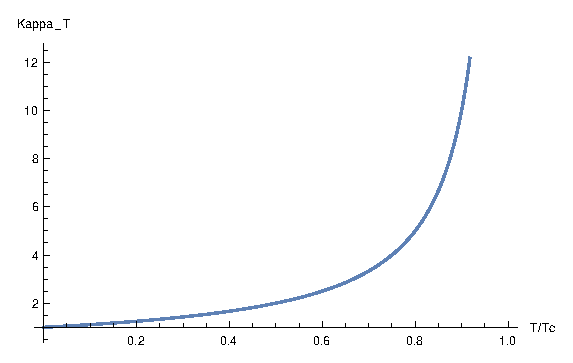
\includegraphics[width=0.5\textwidth]{sketch}
		\caption{Sketch of $\kappa_T$, which diverges at $T_c$.}
	\end{figure}


	\item ``On the critical isotherm'' means keeping $T = T_c$. So this part just asks us to write $P-P_c$ in terms of $n-n_c$, where $n_c = b/2c, T_c = b^2/4ck_B$, and $P_c = b^3/24c^2$
	\begin{align*}
	P - P_c &= \lp nk_BT_c + \f{cn^3}{3} - \f{b n^2}{2}\rp - \f{b^3}{24c^2} \\
	&= -\f{(b-2cn)^3}{24c^2} \\
	&= \boxed{\f{c}{3}(n-n_c)^3}
	\end{align*}
	\item Along an isotherm, variations of chemical potential obey
	\begin{align*}
	d\mu = \f{ d P }{n}
	\end{align*}
	Now, since the chemical potential of the two phases are the same at the phase transition, we have
	\begin{align*}
	\mu(n_+) - \mu(n_-) &= 0 \\
	&= \int\,d\mu \\
	&= \int \f{1}{n} dP \\
	&= \int^{n_+}_{n_-} \f{1}{n}\f{\p P}{\p n}\,dn\\
	&= \int^{n_c(1+\delta)}_{n_c(1-\delta)} \f{1}{n}\f{\p P}{\p n}\,dn \\
	&= \int^{n_c(1+\delta)}_{n_c(1-\delta)}\lb -b + cn + \f{k_B T}{n} \rb\,dn \\
	&= \f{b^2\delta}{2c} + k_BT \ln \f{1+\delta}{1-\delta}.
	\end{align*}
	Mathematica code:
	\begin{lstlisting}
	In[10]:= Integrate[-b + c n, {n, nc (1 + d), 
	nc (1 - d)}] // FullSimplify
	
	Out[10]= (b^2 d)/(2 c)
	\end{lstlisting}
	The implicit equation for $\delta$ is thus
	\begin{align*}
	\boxed{\delta} = \f{2k_B Tc}{b^2}\ln \f{1+\delta}{1-\delta} = \boxed{\f{T}{2T_c} \ln \f{1+\delta}{1-\delta} }
	\end{align*}
	This is a transcendental equation, so we can't solve it analytically. However, we may assume that $\delta \ll 1$ and expand the log to get
	\begin{align*}
	\delta \approx \f{T}{T_c}\lp \delta + \f{\delta^3}{3} + \mathcal{O}(\delta^5) \rp
	\end{align*} 
	Mathematica code:
	\begin{lstlisting}
	In[16]:= Series[Log[(1 + x)/(1 - x)], {x, 0, 4}]
	
	Out[16]= SeriesData[x, 0, {2, 0, 
	Rational[2, 3]}, 1, 5, 1]
	\end{lstlisting}
	
	With this, we can now solve for $\delta$ in terms of $T$ and $T_c$ (assuming $T>T_c$)
	\begin{align*}
	\boxed{\delta \approx \f{\sqrt{3(T/T_c-1)}}{\sqrt{T/T_c}} = \sqrt{3\lp 1 - \f{T_c}{T} \rp}}
	\end{align*}
	Mathematica code:
	\begin{lstlisting}
	In[17]:= Solve[x == r*(x + x^3/3), x]
	
	Out[17]= {{x -> 0}, {x -> -((Sqrt[3] Sqrt[1 - r])/Sqrt[r])}, {x -> (
	Sqrt[3] Sqrt[1 - r])/Sqrt[r]}}
	\end{lstlisting}
\end{enumerate}

\noindent \textbf{4. Quantum-Classical correspondence.} The Hamiltonian says 

\begin{enumerate}[label=(\alph*)]
	\item BCH formula says
	\begin{align*}
	e^{-\be \ham} = e^{-\be p^2/2m} e^{-\be U({q})} e^{-\be^2 [p^2/2m, U({q})]} 
	\end{align*}
	In the high temperature limit, we have $\be^2 [p^2, U({q})] \to 0$, so effectively $p^2$ and $U({q})$ commute, just like in classical mechanics. Not surprisingly, the quantum mechanical partition function will also turn into the classical partition function:
	\begin{align*}
	\mathcal{Z}_\text{QM} 
	&= \Tr\lp e^{-\be \ham}  \rp \approx  \Tr\lp e^{-\be p^2/2m} e^{-\be U({q})} \rp\quad\quad\quad \text{as  }\,\,\be \to 0 \\
	&= \sum_{n}\bra{n} e^{-\be p^2/2m} e^{-\be U({q})} \ket{{n}}\\
	&= \int d^3  \vec{p} d^3 \vec{q} \, \bra{n}e^{-\be p^2/2m} \ketbra{p}  e^{-\be U(\vec{q})} \ketbra{q} \ket{n},\quad\quad \{ \ket{n} \}\text{ is, say, the energy basis}\\
	&= \int d^3  \vec{p} d^3 \vec{q} \,
	e^{-\be p^2/2m} e^{-\be U(\vec{q})} \bra{n}\ketbra{p}   \ketbra{q} \ket{n}\\
	&= \int d^3  \vec{p} d^3 \vec{q}  e^{-\be p^2/2m}  e^{-\be U(\vec{q})} \abs{\bra{p}\ket{q}}^2\\
	&= \f{1}{h^3}\int d^3  \vec{p} d^3 \vec{q}  e^{-\be p^2/2m}  e^{-\be U(\vec{q})}\\
	&= \mathcal{Z}_\text{CM}
	\end{align*}
	where we have used the fact that $\bra{\vec{q}}\ket{\vec{p}} \sim e^{i \vec{p}\cdot \vec{q}}/(2\pi \hbar)^{3/2}       $. 
	
	
	\item For a free particle in a box of volume $V$, we have that the integral over the positional phase space is just $V$. The Hamiltonian is diagonal in the $\vec{k}$ basis as
	\begin{align*}
	\ham \ket{\vec{k}} = \mathcal{E}(\vec{k}) \ket{\vec{k}} 
	\end{align*}
	where $\mathcal{E}(\vec{k}) = \hbar^2 k^2 / 2m$ and
	\begin{align*}
	\bra{\vec{q}} \ket{\vec{k}} = \f{e^{i \vec{k}\cdot \vec{q}}}{\sqrt{V}} 
	\end{align*}
	Let the box be of size $V^{1/3}$, then the allowed values of $\vec{k}$ are $(2\pi V^{1/3}) (l_x,l_y,l_z)$ where the $l_i$'s are integers. The partition function that follows is 
	\begin{align*}
	\mathcal{Z} = \tr(-\be \ham) = \sum_{\vec{k}} \exp\lp -\f{\be \hbar^2 k^2}{2m} \rp
	\end{align*}
	The large-box limit is analogous to the $\be \to 0$ limit, so we may use the result above to say that
	\begin{align*}
	\lim_{V\to \infty}\mathcal{Z} 
	&= \mathcal{Z}_\text{CM} \\
	&= \f{1}{h^3} \int d^3 \vec{p} \exp\lp \f{-\be p^2}{2m}\rp   \underbrace{{\int_V d^3\vec{q}}}_{V} \\
	&= V \int \f{ d^3 \vec{k}}{(2\pi)^3} \exp\lp \f{-\be \hbar^2 k^2}{2m} \rp
	\end{align*}
	where we have used $\vec{p} = \hbar \vec{k} = (h/2\pi) \vec{k}$. From the above two equations we have
	\begin{align*}
	\lim_{V\to \infty} \mathcal{Z}= \lim_{V\to \infty } \sum_{\vec{k}} \exp\lp -\f{\be \hbar^2 k^2}{2m} \rp = V \int \f{ d^3 \vec{k}}{(2\pi)^3} \exp\lp \f{-\be \hbar^2 k^2}{2m} \rp
	\end{align*}
	from which we conclude that
	\begin{align*}
	\sum_{\vec{k}} \to V \int \f{d^3\vec{k}}{(2\pi)^3}
	\end{align*}
	as desired. 
\end{enumerate}

\noindent \textbf{5. Vibrational and rotational heat capacities at high temperatures.}

\begin{enumerate}[label=(\alph*)]
	\item The energy spectrum of a quantum harmonic oscillator is $E_n = \hbar \omega (n + 1/2)$, so the vibrational partition function is 
	\begin{align*}
	\mathcal{Z}_\text{qm,vib} = \sum^\infty_{n=0} \exp\lb -\be \hbar \omega\lp n + \f{1}{2} \rp \rb = \boxed{\f{1}{2}\csch(\f{\be \hbar \omega}{2})}
	\end{align*}
	Expanding $\ln \mathcal{Z}_\text{qm,vib}$ gives
	\begin{align*}
	\boxed{\ln \mathcal{Z}_\text{qm,vib} \approx \ln \lp \f{1}{\be \hbar \omega}\rp - \f{(\be \hbar \omega)^2}{24} + \mathcal{O}((\be \hbar \omega)^3)}
	\end{align*}
	Mathematica code:
	\begin{lstlisting}
	In[3]:= Zq = 
	Sum[Exp[-b*hbar*w*(n + 1/2)], {n, 0, Infinity}] // FullSimplify
	
	Out[3]= 1/2 Csch[(b hbar w)/2]
	
	In[6]:= Series[Log[Zq], {w, 0, 2}]
	
	Out[6]= SeriesData[w, 0, {
	Log[b^(-1) hbar^(-1)/w], 0, Rational[-1, 24] b^2 hbar^2}, 0, 3, 1]
	\end{lstlisting}
	
	
	\item The first correction due to heat capacity due to quantized vibration is
	\begin{align*}
	C = \f{\p E}{\p T} = \f{\p }{\p T}\lb - \f{\p \ln \mathcal{Z}_\text{qm,vib} }{\p \be} \rb = \f{\p }{\p T}\lb k_BT + \f{\hbar^2 \omega^2}{12 k_BT}\rb = k_B - \f{\hbar^2 \omega^2}{12 k_B T^2} \to \boxed{k_B}
	\end{align*}
	as $T\to \infty$. 
	
	\item Checking the Abel-Plana formula. The formula claims that
	\begin{align*}
	\sum^\infty_{n=0} e^{-nu} 
	&= \int^\infty_0 e^{-xu}\,dx + \f{1}{2} + i\int^\infty_0 \f{e^{-iut} - e^{iut}}{e^{2\pi t} - 1}\,dt \\
	&= \f{1}{u} + \f{1}{2} - \f{1}{u} + \f{1}{2}\coth(\f{u}{2})\\
	&=  \f{1}{2} + \f{1}{2}\coth(\f{u}{2}) \\
	&= \f{1}{2} + \f{1}{2}\lp \f{e^u + 1}{ e^u - 1} \rp \\
	&= 1 + \f{1}{e^u - 1} 
	\end{align*}
	while the geometric series $\sum_n e^{-nu}$ is 
	\begin{align*}
	\sum^\infty_{n=0} e^{-nu} = 1 + \f{1}{e^u - 1}.
	\end{align*}
	So, the formula provides the correct expansion for the series above. 
	
	\item Using the formula, we find that 
	\begin{align*}
	\sum^\infty_{l=0} (2l+1) e^{-ul(l+1)} 
	&=   \int^\infty_0 (2x+1) e^{-ux(x+1)} \,dx + \f{1}{2} + i\int^\infty_0 \f{(2it+1) e^{-uit(it+1)}  - (-2it+1) e^{+uit(-it+1)} }{e^{2\pi t} - 1}\,dt \\
	&= \f{1}{u} + \f{1}{2} + i\int_0^\infty \lb 2it (\coth \pi t - 1) + it(2t^2 - 1)(\coth \pi t - 1) u + \mathcal{O}(u^2)  \rb \,dt \\
	&= \f{1}{u} + \f{1}{2} - \f{1}{6} + \f{u}{15} + \mathcal{O}(u^2)\\
	&= \boxed{\f{1}{u} + \f{1}{3} + \f{u}{15} + \mathcal{O}(u^2)}
	\end{align*}
	Mathematica code:
	\begin{lstlisting}
	In[1]:= Integrate[(2*x + 1)*Exp[-u*x (x + 1)], {x, 0, Infinity}]
	
	Out[1]= ConditionalExpression[1/u, Re[u] > 0]
	
	In[2]:= M = (2*I*t + 1)*Exp[-u*I*t (I*t + 1)] - (2*-I*t + 1)*
	Exp[-u*-I*t (-I*t + 1)] // FullSimplify
	
	Out[2]= 2 I E^(t^2 u) (2 t Cos[t u] - Sin[t u])
	
	In[3]:= K = M/(Exp[2*Pi*t] - 1) // FullSimplify
	
	Out[3]= I E^(t^2 u) (-1 + Coth[\[Pi] t]) (2 t Cos[t u] - Sin[t u])
	
	In[4]:= Series[K, {u, 0, 1}] // FullSimplify
	
	Out[4]= SeriesData[u, 0, {
	Complex[0, 2] t (-1 + Coth[Pi t]), 
	Complex[0, 1] t (-1 + 2 t^2) (-1 + Coth[Pi t])}, 0, 2, 1]
	
	In[6]:= I*Integrate[2 I t (-1 + Coth[\[Pi] t]), {t, 0, Infinity}]
	
	Out[6]= -(1/6)
	
	In[12]:= I*
	Integrate[I t (-1 + 2 t^2) (-1 + Coth[\[Pi] t]), {t, 0, Infinity}]
	
	Out[12]= 1/15
	\end{lstlisting}
	
	\item From the lecture notes, the partition function associated with the quantum rotor is 
	\begin{align*}
	\mathcal{Z}_{\text{qm, rot}} 
	&= \sum^\infty_{l=0} \exp
	\lb -\f{\be\hbar^2 l(l+1)}{2I} \rb (2l+1) \\
	&\approx \f{1}{\be \hbar^2/2I} + \f{1}{3} + \f{\be\hbar^2}{30I} \\
	&= {\f{2I}{\be \hbar^2} + \f{1}{3} + \f{\be\hbar^2}{30 I}}
	\end{align*}
	from which we find the energy:
	\begin{align*}
	E_\text{qm,rot} = -\f{\p \ln \mathcal{Z}_{\text{qm,rot}}}{\p \be} = {\f{1}{\be} - \f{2(\be \hbar^4 + 5 \hbar^2 I )}{\be^2 \hbar^4 + 10 \be \hbar^2 I + 60 I^2}}
	\end{align*}
	In the $\be \to 0$ limit, we find that
	\begin{align*}
	E_\text{qm,rot} \to \f{1}{\be} - \f{\hbar^2}{6I} = \boxed{k_B T - \f{\hbar^2}{6I}}
	\end{align*}
	
	
	\item To find the first order correction in rotational heat capacity, we may write
	\begin{align*}
	E_\text{qm, rot} = \f{1}{\be} - \f{2(\be \hbar^4 + 5 \hbar^2 I )}{\be^2 \hbar^4 + 10 \be \hbar^2 I + 60 I^2}  = E_0 + E_1
	\end{align*}
	where $E_0 = 1/\be$. Writing the heat capacity as $C = C_0 + C_1$ where $C_0 = k_B$ we see that the desired correction is 
	\begin{align*}
	C_1 = \f{\p E_1}{\p T} = -\frac{2 \hbar^4 k_B \left(\hbar^4+10 \hbar^2 I
		k_B T -10 I^2 k_B^2 T^2\right)}{\left(\hbar^4+10
		\hbar^2 I k_B T + 60 I^2 k_B^2 T^2\right)^2} \to 0 
	\end{align*}
	as $T\to \infty$. So, the first order correction to the heat capacity due to quantized rotation is $\boxed{k_B}$ as $T\to \infty$. \textbf{\textcolor{blue}{We could have used the expression for $E$ in the high temperature limit -- I'm just being careful here.}}
\end{enumerate}

\noindent \textbf{6. van Leeuwen's Theorem.} The Hamiltonian for a gas of charged particles subjected to an external magnetic field $\vec{B} = \curl \vec{a}$ is 
\begin{align*}
\ham = \sum^N_{i=1} \f{1}{2m}(\vec{p}_i - e\vec{A})^2 + U(\vec{q}_1, \dots, \vec{q}_N).
\end{align*}
We wish to show that the thermodynamics of the problem is independent of $\vec{B}$. To this end, let us consider the partition functions $\mathcal{Z}_0$ and $\mathcal{Z}_{\vec{B}}$ corresponding to the system without and with the external magnetic field. Let us treat this problem classically, as quantum effects are ignored. With this, 
\begin{align*}
\mathcal{Z}_0 
&= \f{1}{h^3} \int \prod^N_{i=1} d^3\vec{p}_i d^3 \vec{q}_i \exp\lb -\be \lp 
\sum^N_{i=1} \f{1}{2m}\vec{p}_i^2 + U(\vec{q}_1, \dots, \vec{q}_N) \rp \rb.
\end{align*}
\begin{align*}
\mathcal{Z}_{\vec{B}}
&= \f{1}{h^3} \int \prod^N_{i=1} d^3\vec{p}_i d^3 \vec{q}_i \exp\lb -\be \lp 
\sum^N_{i=1} \f{1}{2m}(\vec{p}_i - e\vec{A})^2 + U(\vec{q}_1, \dots, \vec{q}_N) \rp \rb.
\end{align*}
By a change of variables $p'_i = p_i - e\vec{A}$, we see that the integration measure in $\mathcal{Z}_{\vec{B}}$ does not change, and the integrand now matches that of $\mathcal{Z}_0$. As a result, we find that
\begin{align*}
\mathcal{Z}_0 = \mathcal{Z}_{\vec{B}}
\end{align*}
for any $\vec{B}$. Therefore, $\mathcal{Z}$ is independent of $\vec{B}$. This implies that the thermodynamic properties of the problem (all of which are derived from $\mathcal{Z}$) are also independent of $\vec{B}$. \\ 




\noindent \textbf{7. (Optional) Zero-point energy.} The Hamiltonian is 
\begin{align*}
\ham_\text{cl} = \f{p^2}{2m} + \f{m\omega^2 q^2}{2}. 
\end{align*}
We will assume that in quantum mechanics the energy levels are quantized as $\ham_\text{qm} = x + yn$ where $n\in \mathbb{Z}$. 

\begin{enumerate}[label=(\alph*)]
	\item The classical partition function is 
	\begin{align*}
	\mathcal{Z}_\text{cl}(\be) = \f{1}{h}\int^\infty_{-\infty}\int^\infty_{-\infty}  dp\,dq\, \exp\lp -\f{\be p^2}{2m} - \f{\be m \omega^2 q^2}{2} \rp =  \f{2\pi}{\be h\omega} = \boxed{\f{1}{\be \hbar \omega}}
	\end{align*}

	
	The energy is 
	\begin{align*}
	E(T) = -\f{\p }{\p \be} \ln \mathcal{Z}_\text{cl} = \boxed{\f{1}{\be}}
	\end{align*}
	
	Mathematica code:
	\begin{lstlisting}
	In[3]:= Z = 
	Integrate[(1/h)*Exp[-b*p^2/(2 m) - b*m*w^2*q^2/2], {p, -Infinity, 
	Infinity}, {q, -Infinity, Infinity}] // FullSimplify
	
	Out[3]= ConditionalExpression[(2 \[Pi])/(h Sqrt[b/m] Sqrt[b m w^2]), 
	Re[b/m] > 0]
	
	In[5]:= En = D[-Log[Z], b] // FullSimplify
	
	Out[5]= ConditionalExpression[1/b, Re[b/m] > 0]
	\end{lstlisting}
	
	\item The quantum partition function is 
	\begin{align*}
	\mathcal{Z}_\text{qm} = \Tr\lp e^{-\be(x+yn)} \rp = \sum_{n=0}^\infty e^{-\be(x+yn)} = {\f{e^{-\be(x-y)}}{e^{\be y} - 1} } = \boxed{\f{e^{-\be x}}{ 1 - e^{-\be y}}}
	\end{align*}
	At high temperatures, we may match $\mathcal{Z}_\text{cl}$ to $\mathcal{Z}_\text{qm}$ to find $y$ by \textcolor{red}{eliminating} $x$ (\textcolor{blue}{this feels very wrong...})
	\begin{align*}
	\lim_{\be \to 0} \mathcal{Z}_\text{qm} \approx \f{1}{ 1 - (1- \be y)} = \mathcal{Z}_\text{cl} = \f{1}{\be \hbar \omega} \implies \boxed{y = \hbar \omega} 
	\end{align*}

	
	
	\item The quantum energy is 
	\begin{align*}
	E_\text{qm} = -\f{\p}{\p \be}\ln \mathcal{Z}_\text{qm} = -\f{\p}{\p \be} \lb \f{e^{-\be x}}{ 1 - e^{-\be y}}  \rb = \boxed{x + \f{y}{e^{\be y} - 1}}
	\end{align*}
	When $\be \to 0$, we may expand $E\text{qm}$ as follows 
	\begin{align*}
	E_\text{qm} \approx \f{1}{\be} + \lp x - \f{y}{2}  \rp + \mathcal{O}(\be)	
	\end{align*}
	Matching this result to $E_\text{cl} = 1/\be$, we find that
	\begin{align*}
	x = \f{y}{2} = \boxed{\f{\hbar \omega}{2}}
	\end{align*}
	so the quantum Hamiltonian is 
	\begin{align*}
	\ham_n = \hbar \omega\lp n + \f{1}{2} \rp
	\end{align*}
	as expected, with $\hbar\omega/2$ being the zero point energy. 
\end{enumerate}

\noindent \textbf{8. (Optional) Quantum mechanical entropy.}

\begin{enumerate}[label=(\alph*)]
	\item The density matrix $\rho(t)$ solves the Liouville's equation, so we have
	\begin{align*}
	\f{d\rho }{dt} = \f{\p \rho}{\p t} + \f{1}{i\hbar} [\rho, \ham] = 0 \implies \boxed{i\hbar \f{\p}{\p t}\rho = [\ham,\rho]}
	\end{align*}
	From here, we can calculate $dS/dt$ as follows:
	\begin{align*}
	\f{dS}{dt} &= -\Tr \lb \f{\p \rho(t)}{\p t}(\ln \rho(t) + \mathbb{I} ) \rb \\
	&= -\f{1}{i\hbar}\Tr\lb (\ham \rho  - \rho \ham)(\ln \rho + \mathbb{I})  \rb\\
	&= \cancel{-\f{1}{i\hbar}\Tr\lb \ham \rho - \rho \ham \rb} + -\f{1}{i\hbar}\Tr\lb \ham \rho \ln \rho - \rho \ham \ln \rho \rb\\
	&= -\f{1}{i\hbar}\lb \Tr(\ham \rho \ln \rho)- \Tr(\ln \rho \rho \ham)  \rb\\
	&= \boxed{0}
	\end{align*}
	where we have used the fact that $\Tr(ABC)$ is invariant under cyclic permutations and that $[\rho,\ln \rho]  = 0$. \textcolor{blue}{I suppose this makes sense, since the quantum time evolution operator is unitary.}
	
	
	\item The functional $S[\rho]$ subject to the constraint $\tr(\rho \ham) = E$ and normalization $\Tr \rho = 1$ is:  
	\begin{align*}
	S[\rho] = \Tr(\rho \ln \rho)  + \be\lb E - \Tr(\rho \ham) \rb + \al[1 - \Tr\rho]
	\end{align*}
	where $\al,\be$ are our Lagrange multipliers. With this, we can extremize $S$ with respect to $\rho$ to find $\rho_\text{max}$:
	\begin{align*}
	\f{\p S[\rho]}{\p \rho}\bigg\vert_{\rho_\text{max}} = \Tr(\ln \rho_\text{max} + \mathbb{I}) - \be \Tr(\ham) -\al \Tr\mathbb{I} = 0
	\end{align*}
	from which we find 
	\begin{align*}
	\ln \rho_\text{max} = -\be\ham - \al\mathbb{I} - \mathbb{I} \implies \boxed{\rho_\text{max} = e^{-(\al + 1)}e^{-\be\ham}} 
	\end{align*}
	To the correct normalization we must have $e^{-(\al + 1)} = \Tr(e^{-\be \ham}) $, but since we started with two Lagrange multipliers we could leave our answer as that in the box. 
	
	
	
	\item Since $\rho_\text{max} = \rho_\text{max}(\ham)$, it commutes with $\ham$. Thus,
	\begin{align*}
	\f{\p \rho_\text{max}}{\p t} = \f{1}{i\hbar} [\ham, \rho_\text{max}] = \boxed{0}
	\end{align*} 
	
	
	
\end{enumerate}

\noindent \textbf{9. (Optional) Electron spin. }

\begin{enumerate}[label=(\alph*)]
	\item When $\vec{B} = B\hat{z}$ we have
	\begin{align*}
	\ham_z = -\mu_B B \sigma_z.
	\end{align*}
	The density matrix for the canonical ensemble is therefore
	\begin{align*}
	\rho_z = \f{1}{\tr(e^{-\be\ham_z })}\exp\lp -\be \ham_z \rp = \boxed{\f{1}{e^{-\be B \mu_B} + e^{\be B \mu_B}}\begin{pmatrix}
	e^{\be B \mu_B} & 0 \\ 0 & e^{-\be B \mu_B}
	\end{pmatrix}}
	\end{align*}
	Mathematica code:
	\begin{lstlisting}
	In[47]:= sz = PauliMatrix[3];
	
	In[48]:= Hz = -mu*B*sz;
	
	In[49]:= rhoz = MatrixExp[-b*Hz];
	
	In[50]:= rhoz = rhoz/Tr[rhoz];
	
	In[58]:= rhoz
	
	Out[58]= {{E^(b B mu)/(E^(-b B mu) + E^(b B mu)), 0}, {0, 
	E^(-b B mu)/(E^(-b B mu) + E^(b B mu))}}
	\end{lstlisting}
	
	\item When $\vec{B} = B\hat{x}$ we have
	\begin{align*}
	\ham_x = -\mu_B B \sigma_x.
	\end{align*}
	The density matrix for the canonical ensemble is therefore
	\begin{align*}
	\rho_x = \f{1}{\tr(e^{-\be\ham_x })}\exp\lp -\be \ham_x \rp = 
	\boxed{\f{1}{2}\begin{pmatrix}
		1 & \tanh(\be B \mu_B) \\ \tanh(\be B \mu_B) & 1 
		\end{pmatrix}}
	\end{align*}
	
	Mathematica code:
	\begin{lstlisting}
	In[62]:= Hx = -mu*B*PauliMatrix[1];
	
	In[63]:= rhox = MatrixExp[-b*Hx]; // FullSimplify
	
	In[64]:= rhox = rhox/Tr[rhox] // FullSimplify
	
	Out[64]= {{1/2, 1/2 Tanh[b B mu]}, {1/2 Tanh[b B mu], 1/2}}
	\end{lstlisting}
	
	\item 
	\begin{align*}
	&\langle \ham_z \rangle = \tr(\rho_z \ham_z) = \boxed{- B \mu_B \tanh(\be B \mu_B )}\\
	&\langle \ham_x \rangle = \tr(\rho_x \ham_x) = \boxed{- B \mu_B \tanh(\be B \mu B)}
	\end{align*}
	which is not surprising as there's nothing to distinguish between which way is $z$ or $x$. 
	
	
	Mathematica code:
	\begin{lstlisting}
	In[66]:= Ez = Tr[rhoz . Hz] // FullSimplify
	
	Out[66]= -B mu Tanh[b B mu]
	
	In[67]:= Ex = Tr[rhox . Hx] // FullSimplify
	
	Out[67]= -B mu Tanh[b B mu]
	\end{lstlisting}
\end{enumerate}




\end{document}














